\documentclass[11pt, letterpaper, titlepage]{article}
\usepackage[utf8]{inputenc}
\usepackage[export]{adjustbox}
\usepackage{geometry}
 \geometry{
 a4paper,
 total={168mm,257mm},
 left=20mm,
 top=15mm,
 includefoot,includehead
 }
\usepackage[backend=biber, style=authoryear, giveninits=true, maxbibnames=25, uniquename=init, maxcitenames=2, hyperref=true, dashed=false]{biblatex}			% Benutze Biber/BibLaTeX zum Zitieren
\addbibresource{main.bib}
\usepackage{caption}
\usepackage{subcaption}
\usepackage{graphicx}
\usepackage{svg}
\usepackage{placeins}
\usepackage[hidelinks]{hyperref}
\usepackage{amsmath}
\usepackage[headsepline]{scrlayer-scrpage}
\usepackage{acronym}

\clearpairofpagestyles %Seitenzahl nicht in der Kopfzeile

\title{MeetEU Project - Team Heidelberg - Team 1 -- \\ Identification and Enhancement of novel Sars-CoV-2 NSP13 Helicase Inhibitors}
\author{Linda Blaier, Paul Brunner, Selina Ernst, Valerie Segatz, and Chlo\'{e} Weiler}
\date{February 2024}

\begin{document}

\maketitle

\ihead{\headmark}
\automark{section}  %Kopfzeile gleich dem Sektiontitel
\cfoot{\pagemark}   %\ofood Seitenzahl rechts

\section{Abstract}
%Although the development of vaccines against Sars-CoV-2 was successful during the recent pandemic, the amount of \ac{FDA}-approved drugs for the therapy of \ac{COVID-19} is still limited to Paxlovid and Veklury, Olumiant and Actemra \cite{FDACOVID}. One possibility to accelerate the development of new therapies for \ac{COVID-19} is to screen already approved drugs for effects against the viral reproduction. In this years MeetEU project, we investigated the NSP13 helicase of Sars-CoV-2 and tried to find compounds that could be repurposed for this therapy, as well as novel compounds that could lead to an effective treatment of Covid19. Using our \textit{in-silico} pipeline (see graphical abstract) enables us to evaluate possible drug candidates, suggest novel structures based on already approved drugs and investigate their toxicity, while being cheaper and less labor intensive than projects limited to wet-lab work.

%The development of innovative therapeutics is essential for managing the \ac{SARS-CoV-2} pandemic. The objective is to identify anti-\ac{SARS-CoV-2} agents as substitutes for vaccines or immune therapeutics that are able to maintain their efficacy despite the virus's high mutation rate. Targeting the \ac{NSP13} helicase is a promising strategy due to its high conservation and indispensability for viral replication as part of the replication and transcription complex \cite{marecki,malone2022structures}. Therefore this project focused on the investigation of drugs that inhibit the NSP13 helicase of Sars-CoV-2 by trying to find compounds that could be repurposed for this therapy, as well as novel compounds that could lead to an effective treatment of \ac{COVID-19}. The proposed \textin{in silico} pipeline, depicted in the graphical abstract, aims to repurpose \ac{FDA}-approved drugs and discover novel compounds with potential as future anti-\ac{SARS-CoV-2} therapeutics.

\newpage
%    Abkürzungsverzeichnis
{\setlength{\parskip}{0.2cm}
\section*{Abbreviations}
    \begin{acronym}[LC-MS/MS23]
        % A B C D E F G H I J K L M N O P Q R S T U V W X Y Z        
        % Abkürzungen
        \acro{MD}{Molecular dynamics}
        \acro{NSP13}{Non-structural protein 13}
        \acro{RTC}{Replication transcription complex}
        \acro{SAscore}{Synthetic accessibility score}
        \acro{ssRNA}{Single-stranded RNA}
        \acro{ZBD}{Zinc binding domain}
        \acro{SARS-CoV-2}{severe acute respiratory syndrome corona virus 2}
        \acro{FDA}{food and drug administration}
        \acro{RAS}{renin-angiotensin system}
        \acro{COVID-19}{coronavirus disease 2019}
        \acro{SARS-CoV-2}{SARSI}

        % Formelzeichen
        
        
        % als benutzt markierte Acronyme    
        
        
    \end{acronym}
}
\newpage


\section{Introduction}
Even though the development of vaccines against SARS-CoV-2 was successful during the recent pandemic, the amount of FDA approuved drugs for the therapy of COVID-19 is still limited to Paxlovid, Veklury, Olumiant, and Actemra (\cite{FDA_COVID}). Improving the landscape of drugs available for treating COVID-19 would be particularly beneficial for people who are at risk of severe illness, as vaccines may not fully prevent infections. The goal of this year's Meet-EU project is to develop a pipeline to identify possible inhibtiors against the SARS-CoV-2 helicase also known as \ac{NSP13}. There are two main reasons as to why this protein is a promising drug target. For one, it is highly conserved among corona viruses, which means that the virus is unlikely to develop resistances against drugs targeting \ac{NSP13} through rapid mutations in the viral genome (\cite{Spratt_2021}). On the other hand, \ac{NSP13} together with other non-structural proteins forms the \ac{RTC}, which is essential for viral RNA synthesis (\cite{Malone_2022}). Therefore, inhibiting \ac{NSP13} would severely hinder the spread of the virus inside the host. 
The protein consists of five domains, namely the \ac{ZBD}, the stalk domain, as well as 1A, 2A and 1B. The latter three make up the catalytic centre of the protein, where RNA and ATP bind (\cite{NSP13_basics}). \\
Computer-aided structure-based drug discovery can be followed to identify possible inhibitors of the \ac{NSP13} helicase. These can then be further investigated in wet-lab settings. This process involves several steps: (1) Identification of possible binding sites, (2) high-trhoughput screening of ligands for how well they bind the respective pocket, followed by (3) the evaluation of the binding pathways, the kinetics, and thermodynamics (\cite{Sledz_2018}). Hereby, focussing this screening on well documented or already FDA approved compounds is very attractive, as this drug repurposing potentially shortents the development period and therefore also the development costs (\cite{Pushpakom_2019}).
\ac{ssRNA}, \ac{SARS-CoV-2}
\subsection*{}
\subsection{Identification of Consensus Binding Pocket}
In drug discovery, the initial step is to investigate the protein structure in order to analyse potential binding sites. These are cavities on the surface or interior of the protein with suitable properties to bind a ligand. The functionality of a binding pocket is determined by its shape and location, but also by the amino acid residues which define its pyhsicochemical characteristics (\cite{Stank_2016}). 
Different experimental and theoretical procedures exist to analyse the druggability of such binding pockets. In this work, we combined three different \textit{in silico} tools, each following a different algorithm. Fpocket (\cite{package_Fpocket}) utilises a geometry-based algorithm based on Voronoi tesselation and sequential clustering to determine potential binding sites. We also implemented P2Rank (\cite{package_P2Rank, package_PrankWeb, package_PrankWeb3}), which is based on a machine-learning algorithm. 
P2Rank assigns structural, physicochemical, and evolutionary features to points on the solvent-accessible surface of a protein. From this information, the machine-learning model is built and used to predict and rank potential ligand binding sites. Lastly, FTMAP (\cite{package_FTMAP}) was used to validate the binding pocket found with the previously mentioned approaches. FTMAP uses docking results of sixteen small molecules differing in polarity, shape, and size to identify binding hot spots with a fast Fourier transform correlation. The most favourable docked confirmations are determined through energy minimisation and clustering processes.
Finally, the results of all three tools were combined to identify a consensus binding pocket of the NSP13 helicase. The resulting coordinates of the consensus binding pocket were then used for molecular docking simulations. 

\subsection{Molecular Docking}
Molecular Docking programs are used to evaluate binding affinities between a potential drug candidate and the target protein. A key aspect of this task is the prediction of the ligand position, orientation, and conformation. Search-based methods approach this task by continuously modifying the ligand pose, while estimating its quality or likelihood (score) and stochastically trying to infer the global optimum of the scoring function. Among the most widely used tools are AutoDock Vina (\cite{Trott.2010}) and Glide (\cite{Halgren.2004}), which mainly differ in their scoring functions. However, such search-based methods are computationally expensive. Therefore, in order to be able to screen large datasets, search-based methods are generally restricted to a previously defined binding pocket (\cite{Corso.2022}). Consequently, potential other binding sites of a ligand are not assessed. Machine learning-based blind docking approaches try to address that problem by stochastically predicting binding pocket and ligand pose based on learned characteristics and aligning them. The most promising results are achieved by using Diffdock (\cite{Corso.2022}), a generative model which applies a reverse diffusion process to the docking paradigm. In this manner, Diffdock iteratively transforms an uninformed noisy distribution over ligand poses defined by the degrees of freedom involved in docking (position, turns around its centre of mass, and twists of torsion angles) into a learned model distribution (\cite{Corso.2022}). Corso \textit{et al.} thereby describe this process as a progressive refinement of random ligand poses via updates of their translations, rotations and torsion angles.

\subsection{clustering of compounds}
In an effort to gain a better understanding of the compounds that emerged from our pipeline, our top scoring compounds from our docking simulation were clustered with those of the teams we were paired with ("Sorbonne5" and "Warsaw1"). Direct comparison of the compounds is made challenging by the fact that different binding sites were chosen by the three teams. Nevertheless, this clustering is still interesting, as it may provide an insight into the structural similarity of compounds that can potentially inhibit the \ac{NSP13} helicase \cite{Spratt_2021}.

%\subsection{Lead Drug Enhancement}
%In order to enhance the binding affinity of our drug candidates and thus their performance, we used AutoGrow4 (Version 4.0.3) \cite{package_Autogrow4} to generate novel compounds. Starting with the best binding compounds of our initial docking simulation with AutoDock Vina as generation zero, multiple new structures are generated by combining sub-structures of the first generation or by passing them through a set of possible chemical reactions after converting them into their respective SMILES codes. All of the generated compounds are ranked by their binding affinity. After passing several filters, the best-performing compounds are used as the seed for the next generation. Using this algorithm, compounds are found, which show higher binding affinities than the first generation. As AutoGrow4 labels all new structures by the path by which they were obtained, we can also evaluate the synthesizability.  

\subsection{Estimation of Toxicity and Synthetic Accessibility}
In addition to determining the activity of novel drug candidates on the therapeutic target, predicition of toxic effects is an indispensible step in drug design to be able to assess the predicted risk vs. benefit ratio of the potential drug \cite{roncaglioni2013silico}. As conventional \textit{in vivo} animal tests are time-consuming, expensive, and ethically controversial, researchers nowadays tend to favour \textit{in silico} methods as they are significantly cheaper and faster than wet expirements and they allow for simultaneous evaluation of large numbers of potential drug candidates \cite{raies2016silico,roncaglioni2013silico}. Therefore, \textit{in silico} toxicity tests are routinely integrated into the early stages of drug discovery in an attempt to minimise late-stage failures in drug design \cite{dearden2003silico}. Moreover, novel drugs must not only ensure the safety of patients but also have the capability for large-scale synthesis in order to one day be commercially viable. For that reason, determination of the synthetic accessibility, that is the ease of synthesis of a chemical compound, is essential for estimating the feasibility of an active compound as a pharmaceutical \cite{boda2007structure}. Therefore, in our pipeline we followed up the identification of the lead compounds that exhibit optimal binding affinity within the consensus pocket with an evaluation of the general toxicity and synthetic accessibility of these compounds to help estimate the suitability of the compounds as real-life pharmaceuticals against \ac{COVID-19}.
%After identifying the lead compounds that exhibit optimal binding affinity within the consensus pocket, an evaluation of the general toxicity and synthetic accessibility of these compounds was performed. This additional step helps estimate the suitability of the compounds as real-life pharmaceuticals against COVID-19. 
 %The Tox-score allows for a general assessment of the predicted risk vs. benefit ratio of the potential NSP13 inhibitors. Moreover, \textit{e}ToxPred allows for an insight into the ease of synthesis, indicated by the \ac{SAscore}. This score reflects the ease and efficiency of producing the molecules in large quantities and consequently their feasibility as potential drugs. 

\subsection{Molecular Dynamics Simulation}
As the last step of our pipeline, a \ac{MD} simulation is conducted using the best-scoring compound as a ligand in the binding pocket of the NSP13 protein. Using GROMACS (Version 2023.3) (\cite{package_GROMACS}), this enables us to interpret the stability of the protein-ligand interaction, as well as to identify important residues for the interaction. Using a given force-field, a set of equations describing different forces between the atoms and residues in the protein and ligand, the movement of all atoms in the system can be simulated and analysed. However, this is only possible in a very limited timeframe with a small time step size. As this process is rather resource-heavy, it has to be conducted on a cluster with access to a GPU. 


\section{Material and Methods}
\subsection{Toxicity and Synthetic Accessibility Prediction using \textit{e}ToxPred}
The general toxicity and synthetic accessibility of the each compound was estimated using the machine-learning tool \textit{e}ToxPred (\cite{pu2019toxpred}). The SMILES files of the Top100 compounds from AutoDock Vina (\cite{Trott.2010}) served as input for the pre-trained model.The toxicity predictor was pre-trained on the FDA-approuved and the KEGG-drug datasets whose compounds were considered non-toxic as well as the TOXNET and the T3DB datasets whose compounds were considered toxic using a deep-belief-network based model. This predictor yields a Tox-score between 0 and 1 and in accordance to the paper, all compounds with a Tox-score below 0.58 were deemed non-toxic. The synthetic accessibility was reflected in a synthetic accessibility score (SAscore) which was obtained by training an extra-trees-based classifier on NuBBE, UNPD, FDA-approuved, and DUD-E-active datasets.

\Subsection{Clustering of Compounds}
Lastly, for a deeper understanding of the potential inhibitors of \ac{NSP13}, the 10 top scoring compounds from \textit{Glide} as well as the top 10 best-docking ligands of the teams "Sorebonne5" and "Warsaw1" were clustered. For one, all 30 compounds were hierarchically clustered based on structural similarity. This was done using the \textit{ChemmineR} package from the \textit{Cheminformatic Toolkit for R} \cite{ChemmineR}. In a first step, the atom pair descriptors for each compound were calculated. These descriptors were then used to calculate a similarity matrix using the Tanimoto coefficient. Substraction of the Tanimoto coefficients from 1 resulted in a distance matrix which was then clustered using the single-linkage method. The resulting heatmap is shown in Figure \ref{hc_structure}.
Secondly, respective compounds were clustered based on their physico-chemical properties. To this end, the \ac{HBD}, the \ac{HBA}, the \ac{MW}, and the \ac{LogP} values were calulcated for each compound using \textit{Open Babel Descriptors} \cite{}. To assess the oral activity and drug-like characteristics of the identified compounds, we applied the filtration criteria outlined in Lipinski's Rule of Five \cite{Lipinski_1997}. The resulting heatmap of the compounds fulfilling this rule is shown in Figure \ref{hc_properties}.  

\section{Results}
\subsection{Top 100 Compounds exhibit low toxicity and high synthetic accessibility}
After identifying the top 100 best-binding ligands through AutoDock Vina, our subsequent analysis focused on evaluating their practical applicability as potential drugs by considering their predicted toxicity and synthetic accessibility. The resulting SAscore and Tox-Score for each compound were visualised in a scatter plot as seen in {Figure \ref{eToxPred}}. 

\begin{figure}[h]
    \begin{center}
      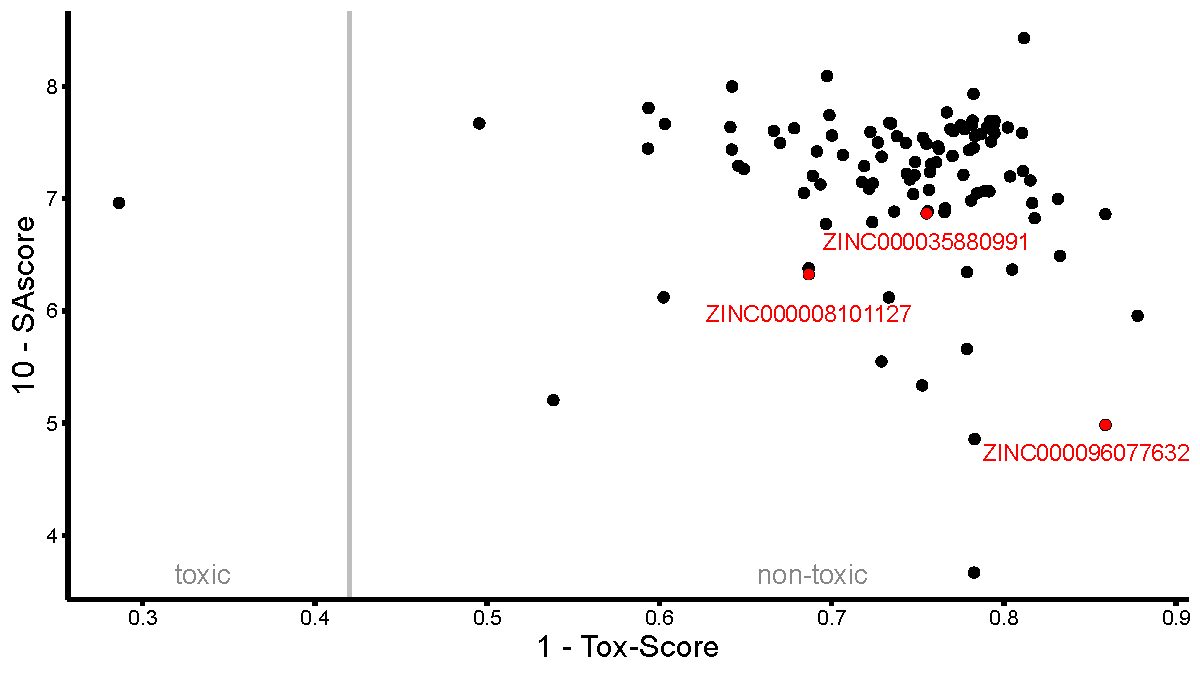
\includegraphics[width=0.9\textwidth]{etoxpred_result.pdf}
    \end{center}
    \caption{\textbf{Scatter plot of predicted toxicity and synthetic accessibility of the 100 best-binding compounds.} The predicted \ac{SAscore} was plotted against the Tox-Score for the top 100 best scorers from AutoDock Vina. The top 3 scorers from Glide are highlighted in red. The vertical gray line represents the threshold for the toxicity, with the compounds to the right of this line being considered non-toxic.}\label{eToxPred}
  \end{figure}

Of those 100 compounds, 99 presented with a Tox-score below the threshold of toxicity, indicating a low probability of being toxic to humans. The overall median Tox-Score is 0.24, with a mean of 0.26 across all compounds. Across all compounds the median SAscore of 2.69 and a mean of 2.87 which suggests that they are genereally easy to synthesise. The top scorer from Glide, ZINC000096077632, was predicted to have a Tox-Score of 0.14 and an SAscore of 5.02.

\subsection{Clustering of compounds}
Comparison of the results from the docking simulations of the three paired teams ("Warsaw1", "Sorbonne5", and "Heidelberg") was performed by clustering the top 30 scoring compounds of the teams based on their structural similarity (Figure \ref{hc_properties} (A)). Here, we can see that the three compounds on ranks 4,5, and 6 from "Sorbonne5" are most dissimilar to each other. Overall the compounds cannot clearly be divided into clusters. This is also reflected in the heatmap that was created based on the physico-chemical properties of the compounds (Figure \ref{hc_properties} (B)). Nevertheless, 22 out of the 30 investigated compounds fulfill Lipinski's Rule of Five. Interestingly, all of the removed compounds share the property that they contain more than 10 \ac{HBA}. Of these compounds, five were detected by team Heidelberg, including our top scoring ligand. The other three compounds came from "Sorbonne5" and none came from "Warsaw1". 
The resulting heatmap of the 22 compounds that fulfill Lipinski's rule and their physico-chemical properties are shown in Figure \ref{hc_properties} (B).  

\begin{figure}
    \centering
    \includegraphics[width=0.6\textwidth]{heatmap.pdf}
    \caption{\textbf{Comparison of the (A) structural and (B) physico-chemical properties of the top scoring compounds from Sorbonne5 (H), Warsaw1 (W), and Heidelberg (H).} The first heatmap(A) is based on the distances of the compounds calculated using the Tanimoto coefficient. In (B) the physic-chemical properties were determined using Open Babel descriptors (\acl{HBD}, \acl{HBA}, \acl{MW}, \acl{logP}). Here, only compounds fulfilling Lipinski's rule of five are shown.}
    \label{hc_properties} 
\end{figure}

\FloatBarrier

\section{Discussion and Outlook}
\subsection{toxicity}
The Tox-Score predictor of \textit{e}ToxPred was trained using \ac{FDA}-approved dataset as non-toxic incidences. Consequently, the low mean Tox-Score of the tested compounds aligns with our expectation, considering that the compounds from the ZINC database are derived from an \ac{FDA}-approved dataset. The single toxic incidence we detected was from the ECBD database which was comprised of \ac{FDA}-approved and non-\ac{FDA}-approved molecules.
As highlighted by \citeauthor{pu2019toxpred}, natural compounds typically exhibit higher \ac{SAscore} values compared to synthetic compounds due to their inherent complexity \cite{pu2019toxpred}. The relatively high \ac{SAscore} of ZINC000096077632 can be explained by the fact that ZINC000096077632 corresponds to angiotensin-(1-7) which is a naturally occuring compound with a crucial role in the \ac{RAS} \cite{santos2014angiotensin}. The analysis of natural compound datasets by \citeauthor{pu2019toxpred} revealed a bimodal distribution in the \ac{SAscore}, with peaks around 3 and 5. Furthermore the very low Tox-Score of the top scorer can also be explained by the fact that it is a naturally occuring molecule in the human body.

\section{Supplementary Material}

\pagebreak
\FloatBarrier
\renewcommand{\bibname}{References}  % damit Literatuverzeicnis mit "References" betitelt
\printbibliography



\end{document}
